\documentclass[main.tex]{subfiles}

\begin{document}

\section{Ray Tracing} \label{section:ray_tracing}

Ray tracing is the designation of a family of algorithms that simulate ray interactions with an environment to determine the visibility of two points in space.
Generally, this technique is used to compute light interactions within a three-dimensional scene, and obtain a two-dimensional image with a rendering of that scene. A high degree of visual realism can be achieved by these techniques, but also with greater computational costs.

Ray tracing algorithms are capable of simulating most optical effects, such as reflections, refractions, and scattering, although the actual set of simulated effects, and their overall quality differ between the multiple ray tracing algorithms that have already been developed.

Large efforts have been made recently to improve ray tracing techniques, with several of them being performance-related, by using parallel architectures such as \gpus, which have always been associated with computer graphics. Some efforts are already showing advances in the area of real time ray tracing, which was unfeasible until very recently \cite{parker2010optix,huss2004real}.


\subsection{Overview}

The first use of ray tracing algorithms was with the introduction of the later called ray casting technique by Arthur Appel in \cite{appel1968some}. The idea consisted of casting one ray from an origin point (usually called the eye, or camera) through each pixel of the image, and find the closest object in the scene that blocks the path of the ray. The material properties and light effects in the scene would then determine the final colour of the pixel.

Later advances (e.g. \cite{whitted2005improved}), introduced the recursive ray tracing algorithm. In traditional ray casting, each ray would end after the first hit. This was a limiting factor that prevented the rendering to deal with reflections. Recursive ray tracing solves that, by recursively tracing more rays after each hit. When a ray hits a surface, it can generate new reflection or refraction, depending on the properties of the material hit. Shadow rays can also be cast in the direction of the light sources. If a shadow ray is blocked by an opaque object before reaching the light source, it means that surface is not illuminated by that light source, and thus is shadowed. This technique is illustrated in \cref{fig:ray_tracing}

\begin{figure}[!htp]
  \centering
  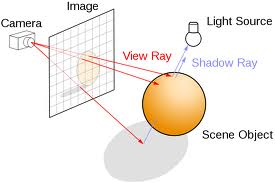
\includegraphics[width=0.5\textwidth]{ray_tracing01}
  \caption[Ray Tracing]{Ray Tracing (from Wikipedia)}
  \label{fig:ray_tracing}
\end{figure}

It is also not uncommon to approximate the rendering equation by using combinations of more than one method, such a Ray Tracing, Radiosity or Metropolis Light Transport \cite{wallace1987two,veach1997metropolis}. Each method attempts to simulate the travel of light particles across the scene, and model the various interactions with the environment, but with different approaches, advantages and limitations, so the combination of multiple method can combine the advantages of each one.

Traditional ray tracing methods work by simulating light particles traveling from the eye into the scene, being reflected and refracted until they reach a light source. Nowadays, most ray tracing rendering algorithms are in fact bidirectional, having photons shot from the light sources and their interactions computed in addition to regular eye paths.

Radiosity follows an opposite approach, and simulates the path light takes from the light source, until it reaches the eye. It only deals with diffuse interactions, however, and is commonly used in combination with other techniques.

\itodo{proença: fazer a ponte para o photon mapping?}

\subsection{The Rendering Equation}

The realistic simulation of illumination of an environment is a complex problem. In theory, a simulation is truly realistic when it completely simulates, or closely approximates, the rendering equation.

This equation, first proposed in 1986 \cite{kajiya1986rendering}, is based on the laws of conservation of energy, and describes the total amount of emitted light from any given point, based on incoming light and reflection distribution. The equation is presented in \cref{eq:render}

\common{equations/rendering}

In short, the equation defines the surface radiance $\surfaceRadiance$, leaving the point $x$ in the direction $\radianceDir$. This is given by $\emittedLight$, which represents light self-emitted by a surface, and $\incidentLight$, which is the radiance along a given incidence direction. $\brdf$ is the \acf{BRDF} and $\Omega$ represents the semi-sphere of incoming directions centered in $x$.

\end{document}
